\begin{figure}[!t]
\centering
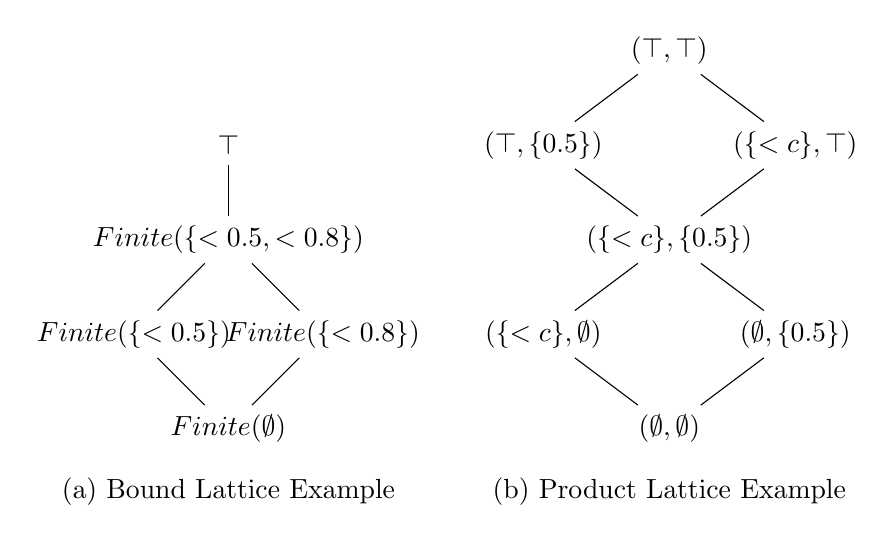
\begin{tikzpicture}[scale=0.8]
  % Individual lattice (left)
  \node (bot1) at (0,0) {$\text{Finite}(\emptyset)$};
  \node (s1) at (-1.5,1.5) {$\text{Finite}(\{<0.5\})$};
  \node (s2) at (1.5,1.5) {$\text{Finite}(\{<0.8\})$};
  \node (s12) at (0,3) {$\text{Finite}(\{<0.5, <0.8\})$};
  \node (top1) at (0,4.5) {$\top$};
  
  \draw (bot1) -- (s1);
  \draw (bot1) -- (s2);
  \draw (s1) -- (s12);
  \draw (s2) -- (s12);
  \draw (s12) -- (top1);
  
  \node at (0,-1) {(a) Bound Lattice Example};
  
  % Product lattice (right)
  \node (bot2) at (7,0) {$(\emptyset, \emptyset)$};
  \node (b1v0) at (5,1.5) {$(\{<c\}, \emptyset)$};
  \node (b0v1) at (9,1.5) {$(\emptyset, \{0.5\})$};
  \node (b1v1) at (7,3) {$(\{<c\}, \{0.5\})$};
  \node (topb) at (5,4.5) {$(\top, \{0.5\})$};
  \node (topv) at (9,4.5) {$(\{<c\}, \top)$};
  \node (top2) at (7,6) {$(\top, \top)$};
  
  \draw (bot2) -- (b1v0);
  \draw (bot2) -- (b0v1);
  \draw (b1v0) -- (b1v1);
  \draw (b0v1) -- (b1v1);
  \draw (b1v1) -- (topb);
  \draw (b1v1) -- (topv);
  \draw (topb) -- (top2);
  \draw (topv) -- (top2);
  
  \node at (7,-1) {(b) Product Lattice Example};
\end{tikzpicture}
\caption{Lattice structure for float types. (a) shows an example bound lattice with comparison bounds. (b) shows the product lattice combining bounds and values.}
\label{fig:lattice}
\end{figure}